\chapter{Systemarchitektur}
Dieser Abschnitt erklärt die Systemarchitektur des Datenhandschuhes, welche Sensoren verwendet, Prozessor-Board gewählt und was für Module verwendet wurden um den Datenhandschuh betriebsfähig zu bauen. Darüber hinaus werden die einzelnen mechanischen Komponenten, die in den Handschuh modelliert genauer Beschrieben.

\section{Systemarchitektur der früheren Version}
Vor dieser Systemarchitektur sollte der frühere Prototyp vorgestellt werden. Paul Bienkowski und Carolin Konietzny haben 2017 den Vorgänger Prototypen entwickelt. Das Hauptziel dieser Arbeit war das entwickeln eines alternativen Eingabegerätes aus einen Datenhandschuh basiert aus IMUs. Mit Hilfe von Maschinellem Lernen entwickelten sie einen System, welches erlaubt das Tippen von zwei Tasten mit einer Genauigkeit von 97\%. Sowie das tippen von 10 Tasten mit drei Fingern eine Genauigkeit von 85\% erreichte. Für diese Arbeit ist jedoch die Systemarchitektur von Bedeutung. 
\begin{figure}[h]
	\centering
    \includegraphics[height=100pt]{Bachelorarbeit/images/PaulBienkowski.png}
    \caption{Prototyp eines Datenhandschuh von Paul Bienkowski und Carolin Konietzny}
    \label{fig:Bienkowski}
\end{figure}

Die Verwendeten Hardware/System Komponenten und Begründungen der Auswahl lauten wie folgt:
\begin{itemize}
    \item Sensor: Der IMU BNO055 wurde wegen seiner Größe des Breakout Boards von $10 x 10mm$ und seinem ausgeprägten integrierten Fusionmodus, welches es erlaubt direkt über den Sensor Orientierung als Quaternion oder Euler-Winkel auszugeben.
    \item Prozessor-Board: Die Auswahlkriterien des Prozessor lagen im Bereich des Formfaktors, hierfür wurde der $Adafruit Feather M0 WiFi$ ausgewählt. Mit einer Größe von $5.4 x 2.3 cm$ und dem Gewicht von $6.1 g$ hat der Prozessor eine gute Form zum befestigen an den Handschuh. 
    \item Ein Shield für die Ansteuerung der Sensoren über die \iic Verbindung
    \item Datenübertragung über die USB-Schnittstelle und den netzwerkbasierten Modus via UDP Pakete.
\end{itemize}
Diese Komponenten sind ausschlaggebend für die Gebräuchlichkeit des Datenhandschuhes, sie sind passend in der Größe, haben die wichtigsten Funktionen und beweisen mit ihrer Datenrate von 90 Hz dass dieser für die allgemeine Verwendung stabil ist. 
\begin{figure}[h]
	\centering
    \includegraphics[height=200pt]{Bachelorarbeit/images/DatenqualitätBienkowski.png}
    \caption{Datenqualität des Datenhandschuh von Paul Bienkowski und Carolin Konietzny}
    \label{fig:DatenqualitätBienkowski}
\end{figure}

Die Qualität beim drücken der Tasten N und H in der Abbildung \ref{fig:DatenqualitätBienkowski} zeigt eine Abweichung von ca. 0.2 Radius, welches für einen Prototypen eine sehr zufriedenstellendes Ergebnis vorweist.

\newpage


\section{IMUs - MPU-6050, BMI160, MPU-9250}
In dieser Abschlussarbeit werden insgesamt drei verschiedene IMU Sensoren verwendet, der MPU-6050, BMI160 und der MPU-9250. Einige wichtige Punkte welche die Sensoren erfüllen sollen ist die Genauigkeit der Daten, die Passfähigkeit für den Handschuh, Einfachheit der Integration und eine Stabile Verbindung zum Host-PC. Für den Gebrauch der Sensoren mussten Modelle verwendet werden, welche geeignet sind für die Finger, diese sollten eine gute Größe besitzen um die Bewegungsfreiheit nicht zu Beeinträchtigen.
\\
\\
Der BMI160 ist ein Modul welches dafür ausgerichtet ist mit niedriger Spannung eine stabile, geräuschlose Datenmessung zu ermitteln. Als Entwurf für mobile Geräte, Augmented Reality oder auch Indoor Navigation entwickelter Sensor, läuft dieses Modul 
\begin{wrapfigure}{r}{0.3\textwidth}
  \begin{center}
    \includegraphics[width=0.18\textwidth]{Bachelorarbeit/images/BMI160.png}
  \end{center}
  \caption{BMI160}
\end{wrapfigure}
mit einer 16 bit digital Auflösung für den Accelerometer und den Gyroscope, für eine genauere Analyse und bestimmte Werte Ausgabe ist es möglich für den Gyroscopen die Maßstäbe benutzerspezifisch auf +-125 +-250, +-500, +-1000 und +-2000° dps, sowie die Accelerometer Maßstäbe auf +-2g, +-4g, +-8g und +-16g zusetzen. Das Modell hat eine original Größe von $2.5 x 3.0 x 0.8mm$ und mit der Paketgröße $18 x 13 x 1.9mm$, ist es das kleinste Modul von den dreien. Ansteuerung des Interface kann mit \iic oder SPI erstellt werden, die SPI läuft mit max. 10 MHZ, während die \iic Schnittstelle nur mit max. 1000 kHZ läuft, die verwendete Adresse des \iic Interface ist standardmäßig $0x68$ und user spezifisch auch $0x69$. Der BMI160 ist somit ein kleiner und stabiler IMU, welcher passend auf dem Fingerrücken befestigt werden kann. 
\\
\\
Die verwendeten InvenSense Modelle MPU-6050 und der MPU-9250 sind zwei sehr ähnliche Modelle. Der MPU-6050 ist ein leistungsstarker Sensor, welcher einen 3-Axis Gyroskop, 3-Axis Accelerometer und einen DMP kombiniert. 
Zudem besitzt 
\setlength\parfillskip{0pt}\par\setlength\parfillskip{0pt plus 1fil}
\begin{wrapfigure}{l}{0.3\textwidth}
  \begin{center}
    \includegraphics[width=0.18\textwidth]{Bachelorarbeit/images/6050.png}
  \end{center}
  \caption{MPU-6050}
\end{wrapfigure}
das Modul drei 16-Bit analog-zu-digital Konvertierer, für den Gyroskop einmal und den Accelerometer, für eine genauere Analyse und Werteausgabe ist es wie beim vorherigen Modul möglich, die gleichen Maßstäbe zu ändern, mit einzigen Unterschied, das der Gyroskop nicht in der Lage ist den Gradwert auf +- 125° zusetzen.
Die original Größe ist fast 1,5-mal so groß wie der BMI160, mit den Maßen  $4 x 4 x 0.9 mm$ und der Paketgröße von $21.2 x 16.4 x 3.3 mm$, aber trotzdem passend für die Finger. 
Der Größen unterschied der BMI160 und MPU-6050 ist somit erkenntlich und für die Verwendung auf dem Fingerrücken mit einzukalkulieren, dieser kann sich nämlich in der Bewegungsfreiheit auswirken. 
Die Ansteuerung des IMUs ist nur mit dem \iic  Interface möglich, welcher auf der höchsten Leistung mit max. 400 kHz auf allen Registern läuft. Hierbei ist die Adresse genau wie im BMI160 auf $0x68$ und userspezifisch $0x69$ gelegt. 
Beide IMUs haben ideale Größen und Eigenschaften, um diese als Fingersensoren zu verwenden, jedoch sind die MPU Modelle Leistungsstärker als die Bosch Sensoren, das kann sich stark auf die Taktrate beim erfassen und bearbeiten der Daten auswirken. Um eine definiertere Datenerfassung der Handbewegung zu ermitteln sind die Finger nicht die einzigen Körperteile, die gemessen werden sollten, hierbei ist auch die Mittelhand sehr wichtig. Aus dieser Position kann der Winkel der Hand besser geschätzt werden, da die Position und der Winkelgrad der Finger die komplette Hand Ausrichtung nicht einfach ermitteln kann.
\setlength\parfillskip{0pt}\par\setlength\parfillskip{0pt plus 1fil}
\begin{wrapfigure}{r}{0.3\textwidth}
  \begin{center}
    \includegraphics[width=0.13\textwidth]{Bachelorarbeit/images/9250.png}
  \end{center}
  \caption{MPU-9250}
\end{wrapfigure}
Die DoF Bestimmung der Gelenke hilft bei der Festlegung der Rotation für die Finger vom Zeigefinger bis zum kleinen Finger, denn diese vier Finger können sich nur in zwei Richtungen bewegen, somit können diese Daten mit der relativen Position der Mittelhand gemessen werden. 
Die Daumen und die Mittelhand besitzen jeweils 3 DoF und können somit auch die z-Achse mit berechnen, da der MPU-9250 auch Magnetometer Daten übermittelt, war somit die Entscheidung diesen für die Mittelhand zu verwenden, damit die Sensorfusion in Relation der Beschleunigung und Winkelgeschwindigkeit einen weiter Faktor zur Stabilisierung erhält und eine bessere, stabile Handposition ausgibt.
\\
\\
Die MPU-9250 ist eine Zusammensetzung des MPU-6500 und dem AKM-8963 die mit dem AUX-\iic des MPU-6500 verbunden sind. Der MPU-6500 unterscheidet sich weniger zum MPU-6050, die Funktionalität ist fast gleich, jedoch hat der MPU-6500 einige Eigenschaften mehr. Der MPU-9250 erlaubt somit auch eine SPI Verbindung mit max. 1 MHz. Mit dem integriertem AKM-8963 ist es auch Magnetometer werte zu messen, welcher die mit der Adresse $0x0C$ ablesbar ist. 
Zu erkennen ist auch das Paul Bienkowski den InvenSense MPU-9150 evaluiert hatte, welche ein Vorgänger der MPU-9250. Diese hat nämlich den MPU-6050, die in dieser Arbeit als Fingersensor verwendet werden ist Leistungsstärker als der verwendeten BNO055 und erlaubt eine höhere Bitrate für den Accelerometer. Die Magnetometer werte entnimmt dieser aus dem AK8975, welcher nur eine Skalierung von +-2048 erlaubt.

\newpage
\section{Prozessor-Board - ESP32}
Die Größe und das Gewicht sollten die Hand nicht behindern oder beeinträchtigen, somit ist wichtig, was für Prozessor-Boards für die beiden Datenhandschuhe verwendet werden.
Hierbei wurde der ES32 für die Architektur ausgewählt. Für den Datenhandschuh relevanten Daten ist der Taktfrequenzbereich von 80 MHz/240 MHz, RAM von 512 kB, \iic Schnittstellen, eine Größe von $48x26x5mm$, Wireless Funktion mit einer Frequenz von 2,4 GHz und einem Verpackungsgewicht von ca. 0.011 kg. Mit seiner Leichtigkeit ist es somit unproblematisch diesen an das Handgelenk zu befestigen, ohne das es unangenehm oder die Bewegungsfreiheit stört.


\section{Multiplexer und Verwendung des \iic}\label{MUX}
Die Ansteuerung der sechs IMUs an dem ESP32 wurde mithilfe eines Multiplexers \textit{TCA9548A} ausgeführt. Der Grund, weshalb nur die \iic Ansteuerung angestrebt wurde, lag an der Vereinheitlichung beider Handschuhe. Da der MPU-6050 nur eine \iic Verbindung erlaubt, stellte sich also die Frage, wie man am besten sechs IMUs an den Prozessor-Board anschließt. 
Der ESP32 besitzt nur einen SDA und SCL Port, welches es bei den IMUs, welche alle die gleiche Adresse teilen, komplizierter gestaltet eine Verbindung herzustellen. 
Um dieses Problem zu lösen bietet der \textit{TCA9548A} eine passende Lösung. Durch seine acht Kanäle erlaubt dieser uns mehrere \iic Anschlüsse mit der gleichen Adresse anzusteuern. 
Die Verbindung wird unkompliziert erstellt und durch die einfache Programmierung gut gestaltet. Die \iic Busses vom ESP32 werden als Master an den MUX angeschlossen, durch die acht Ports werden anschließend die Slaves erreicht.
Wechsel der Kanäle wird durch den Adressen Aufruf des \textit{TCA9548A} hergestellt, hierbei wird auf den Register $0x70$ gewiesen. Die $AD0$, $AD1$ und $AD2$ Ports erlauben das wechseln der Adresseingänge auf $0x70 - 0x77$, was auch einen Anschluss von insgesamt 64 Modulen erlaubt mit der selben Adresse, jedoch wird diese Funktion nicht notwendig. Dieses Vorgehen erlaubt somit eine einfachere Umgehensweise mit dem limitiertem \iic Anschluss.
Das Aufrufen der verschiedenen Ports wird wie folgt ausgeführt:
\begin{lstlisting}
#define TCAADDR 0x70

void tcaselect(uint8_t i) {
  Wire.beginTransmission(TCAADDR);
  Wire.write(1 << i);
  Wire.endTransmission();
}
\end{lstlisting}
Mit \lstinline{tcaselect(uint8_t i)} wird der jeweilige Port auf dem MUX gewählt. Mit der erlaubten höchst Clock Frequenz von 400 kHZ, sollte dieser die Performance nicht beeinträchtigen. Die Verkabelung der IMUs an den Multiplexer werden auf beiden Händen identisch angeschlossen, für parallele Entwicklung. Der \textit{TCA9548A} erlaubt 8 direkt Anschlüsse, somit werden zwei Ports frei stehen und können durch zukünftige Weiterentwicklung verwendet werden, ohne dass die Programmierung beeinflusst wird. \\
Die Verwendeten Ports werden für beide Hände wie folgt unterteilt:
\begin{center}
    \begin{tabular}{  p{3cm} | p{1cm} | p{1cm} | p{1cm} | p{1cm} | p{1cm} | p{1cm} | p{1cm} | p{1cm} }
    \hline
    Ports & 0 & 1 & 2 & 3 & 4 & 5 & 6 & 7 \\ \hline
    Rechts/Links & MH & TH & IF & MF & RF & LF & - & - \\
    \end{tabular}
    MH = Mittelhand, TH = Daumen, IF = Zeigefinger, \\
    MF = Mittelfinger, RF = Ringfinger, LF = Kleiner Finger
\end{center}



\section{Verwendung von Batterie/Akku}
Für die Verwendung des Datenhandschuhes über die Netzwerk Schnittstelle wurde eine Polymer Lithium Ion Batterie $900 mA$ eingesetzt.
Der Einsatz dieser Batterie benötigt ein Lademodul, um die Spannungsversorgung und Lade-/Entladestrom zu regulieren. Der DEBO 4IN1 erlaubt eine kontrollierte Stromzufuhr zwischen Lithium Ion Batterie und dem ESP32, mit seiner Lade, Entlade, Schutzschaltung und Spannungswandlungs Funktion übernimmt dieser hauptsächlich alle benötigten Kriterien der Batterie Verwendung. Durch die integrierten LED Lichter wird der aktuelle Akku Stand angezeigt, sowie die Ladefunktion im Betrieb und mit der Möglichkeit einen Knopf zu befestigen ist dieser in der Lage die Batterie Funktion zu schließen, um nur bei Operation des Handschuhes den Akku zu verwenden.
Der Verbrauch der Module ist abhängig vom deren verwendeten Modus und werden in diesem Fall mit ihrem maximal Ampere definiert. 
\\
\\
Der BMI160 verwendet durch seine Energieeffizient maximal $990${\textmu}$A$, im vollen Betrieb der fünf Gyroskope und Beschleunigungssensoren ist der totale Ampere Verbrauch $990${\textmu}$A x 5 = 4,95 mA$.
Der Verbrauch des MPU-6050 ist durch seine stärkere Funktion höher als der BMI160, mit $3,8 mA$ verbraucht dieser insgesamt $3,8 mA x 5 = 19 mA$, somit ist der Verbrauch fast viermal so hoch wie der BMI160. Der MPU-9250 verwendet mit dem Magnetometer insgesamt $3,7 mA$. Der Prozessor hat bei einem Spannungsbetrieb von $3.3 V$ einen Verbrauch von $40 mA$ und die angeschlossenen LED Lichter beim Betrieb einzeln $20mA$, welches beim dauerhaften Betrieb insgesamt $120 mA$ benötigt.
Beim vollen Betrieb aller Module verwendet der Datenhandschuh mit dem BMI160 insgesamt
$$4,95mA + 3,7mA + 40mA + 120mA = 168,85 mA$$,
somit hält die Polymer Batterie im Dauerbetrieb ca. 6 Stunden ohne Aufladung und mit dem Gebrauch des MPU-6050
$$19mA + 3,7mA + 40mA + 120mA = 182,7mA$$
ca. 5 Stunden. Jedoch ändern sich diese Werte, abhängig von der Verwendung des ESP32, da dieser mit standardmäßigen Programmen bis zu $80 - 170 mA$ verbraucht und bei Verwendung des WiFi Moduls sogar bis zu $400mA$ erreichen kann. 





\newpage

\section{Handschuh Architektur}
Abbildung \ref{fig:GloveArchitektur} zeigt die grundlegende Architektur des Datenhandschuhes. Bis auf die LED Lichter und der Lithium Batterie, welche für die Datenübertragung irrelevant sind, wurden hier alle Komponenten berücksichtigt. 
\begin{figure}[h]
	\centering
    \includegraphics[width=1\columnwidth]{Bachelorarbeit/images/Handarchitektur1.png}
    \caption{Schaltplan des Datenhandschuh - die Architektur mit dem BMI160 ist identisch zu dieser}
    \label{fig:GloveArchitektur}
\end{figure}

Abschnitt \ref{MUX} beschrieb die Verbindung der IMUs zum \textit{TCA9548A}, welcher an die einzigen SDA und SCL Pins des ESP32 befestigt wurden, an den Pins 21 und 22. Für die Verkabelung wurden alle Kabel ausgehend vom GND Pin miteinander gelötet und an den GND Pin des ESP32 befestigt, das gleiche wurde an den VCC Verbindungen gemacht. Die Kabeln wurden lang gehalten, um bei Benutzern mit längeren Fingern keine Behinderung der Bewegung auszulösen. Die Fingerhalterung wurde als einzelnes, trennbares Stück entwickelt\ref{fig:Extractable}, welches es den Benutzer erlaubt, nach der persönlichen Fingergröße die Fingerhalterung zu wechseln oder zu verlängern. Dieses wurde mit Hilfe von Nähband Klettband modelliert.

\begin{figure}[h]
	\centering
    \includegraphics[width=1\columnwidth]{Bachelorarbeit/images/Extractable.jpg}
    \caption{Fingerhalterung gelöst vom Handschuh}
    \label{fig:Extractable}
\end{figure}


Das Anbringen der IMUs an den Fingern wurde mithilfe von angenähten Fächern bewerkstelligt, welches durch das tragen auf den Fingern mit dem Gummiring noch stabiler gestaltet. Die LED Lichter wurden über die IMUs befestigt, jedoch wurden die VCC und GND Verbindung separat gelötet, um diese individuell anzusteuern. Der MPU-9250 wurde mit dem \textit{TCA9548A} auf dem Handrücken angebracht, wegen begrenzten Platz auf dem Handschuh. 

\begin{figure}[h]
	\centering
    \includegraphics[width=1\columnwidth]{Bachelorarbeit/images/IMUswithLEDs.jpg}
    \caption{IMUs und LEDs verbunden}
    \label{fig:IMUSolo}
\end{figure}
Die IMUs und LEDs wurden gemeinsam mit Isolierband verbunden, um stabileren Halt zu geben. Diese sind leicht auswechselbar, schützen vor äußeren Einwirkungen, wie Wasser und geben den Kabeln festen Halt ohne das diese sich durch Bewegungen direkt entkoppeln könnten. 

\begin{figure}[h]
	\centering
    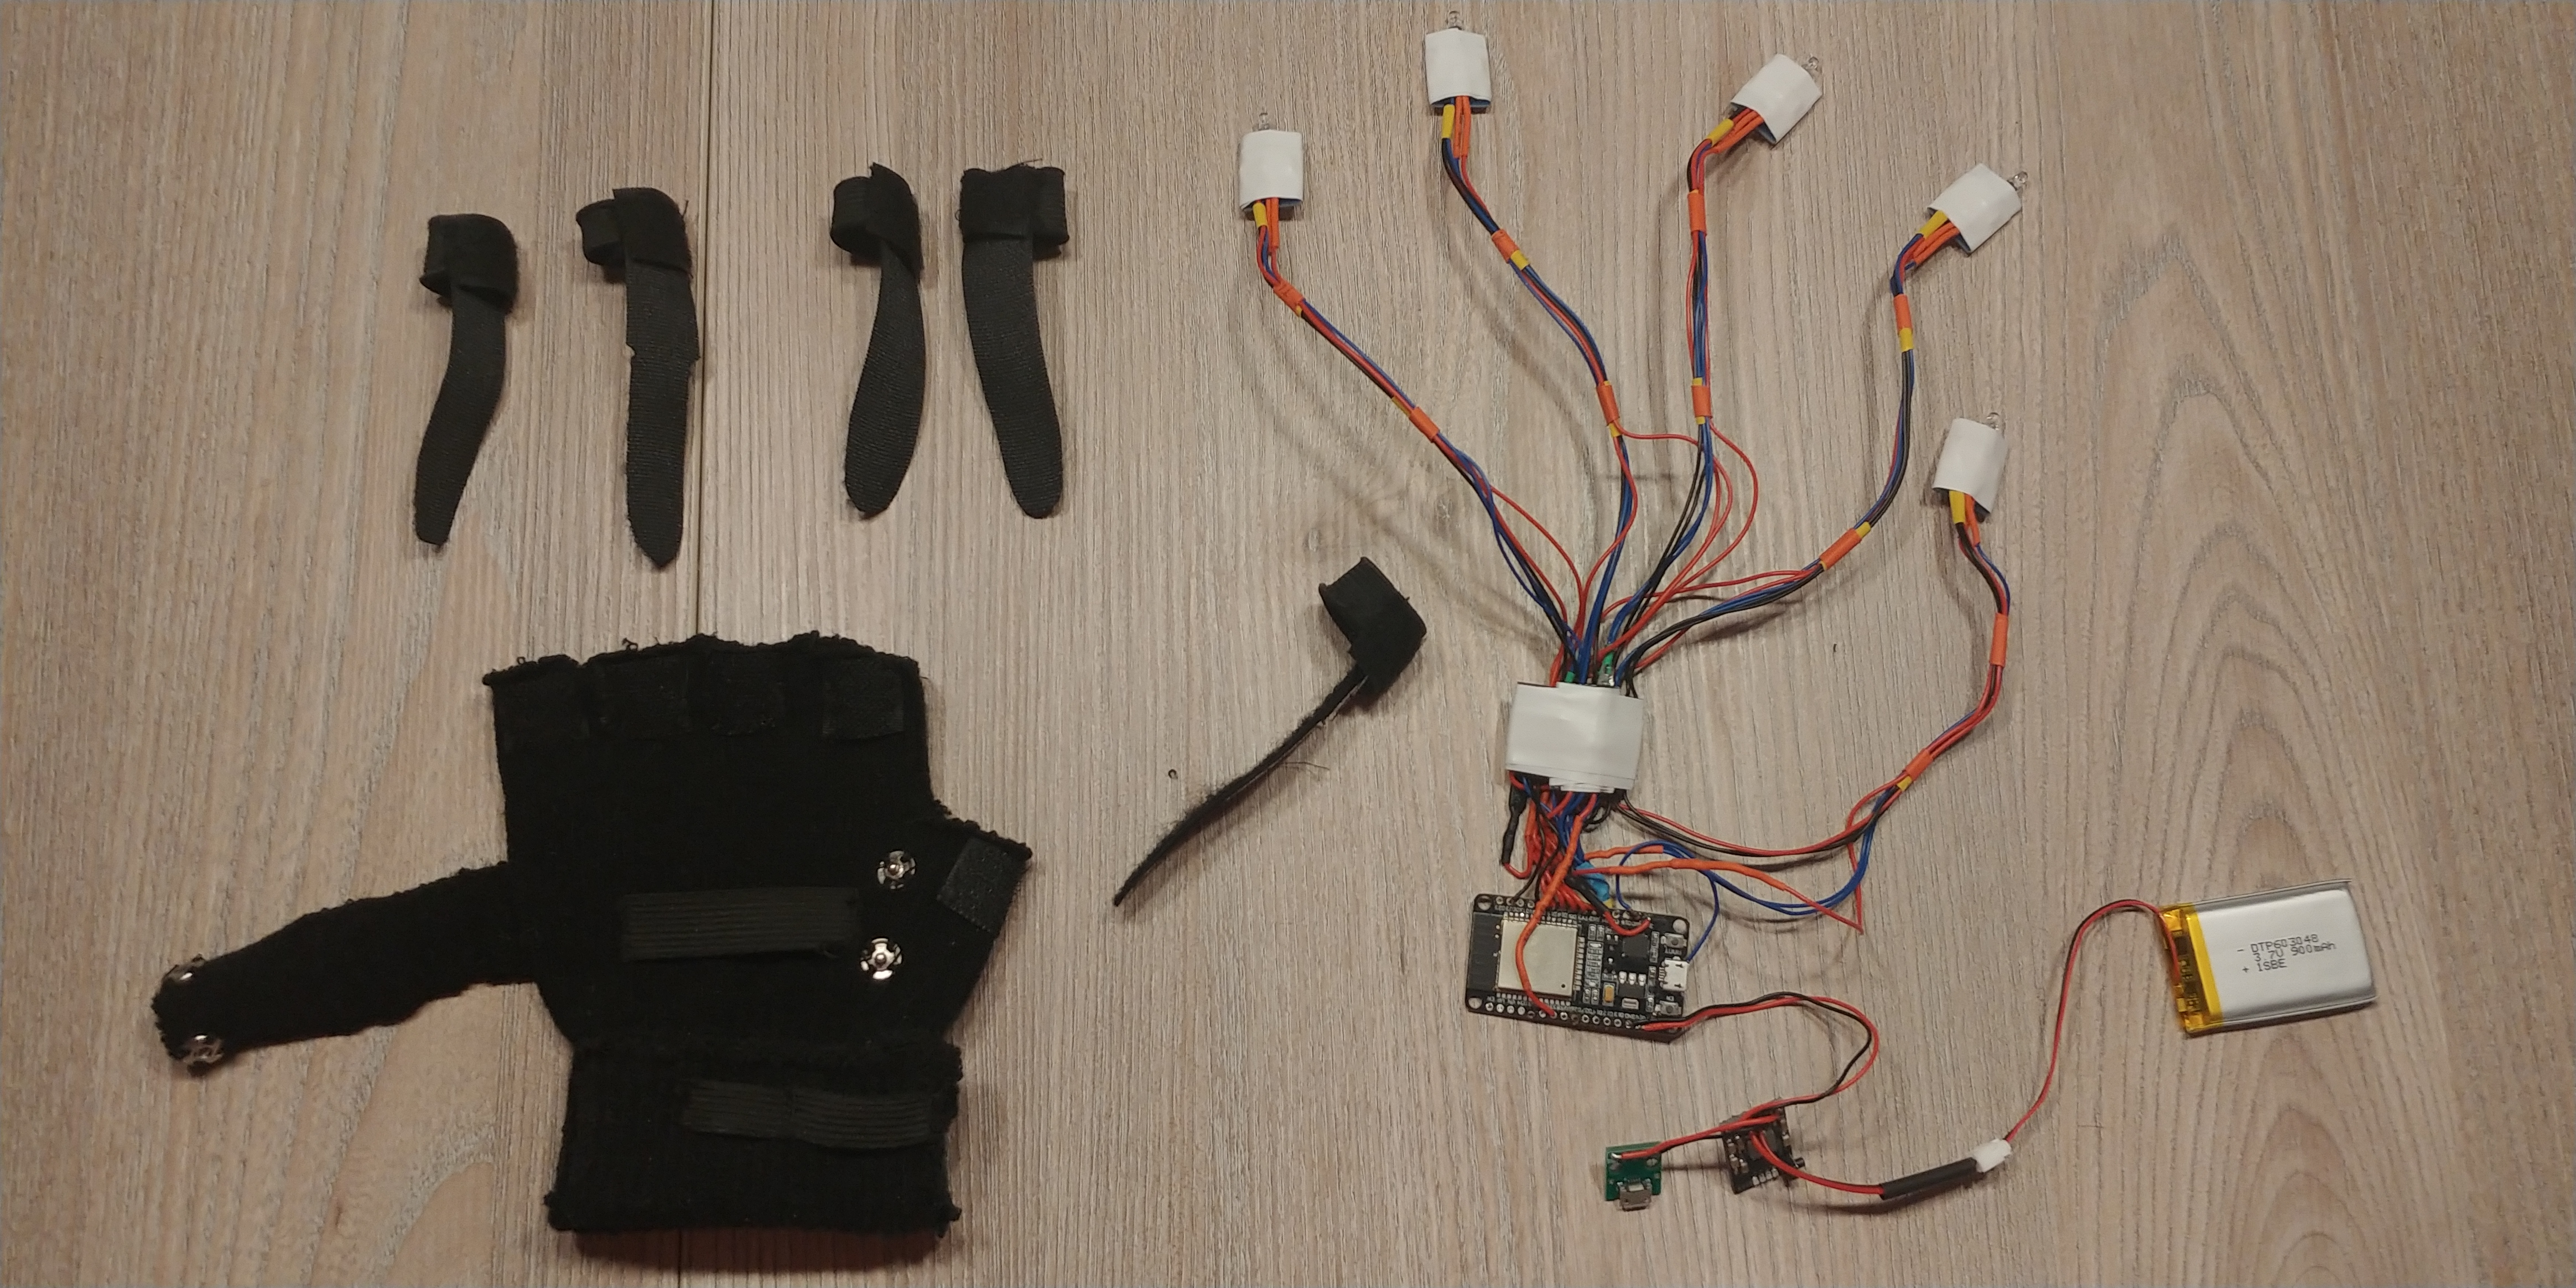
\includegraphics[width=1\columnwidth]{Bachelorarbeit/images/Exo.jpg}
    \caption{Handschuh neben dem Exoskelett und den lösbaren Fingerhalterungen}
    \label{fig:Exo}
\end{figure}

\begin{figure}[h]
	\centering
    \includegraphics[width=1\columnwidth]{Bachelorarbeit/images/FullView.jpg}
    \caption{Komplett Ansicht des Datenhandschuh}
    \label{fig:FullView}
\end{figure}
